% Zum Setzen von TeX-Quellcode, der nicht interpretiert werden soll
\newcommand{\makro}[1]{\texttt{\textbackslash{}#1\{\}}}

\chapter{The TAS-package}
\label{sec:tas_package}

This chapter will show you how to install the TAS-package on the car and give you some details about the different components. The package contains several self-written nodes and launchfiles to run the hardware (Laserscanner, IMU, Arduino) and the so called Navigation Stack properly on the car. The Navigation Stack provides tools for high level tasks like path planning and localization. The TAS-package also brings some shell scripts to make the work a little more comfortable. The folder structure can be seen in picture \reffig{tas_folder_struct}.

\begin{figure}[htbp]
	\centering
		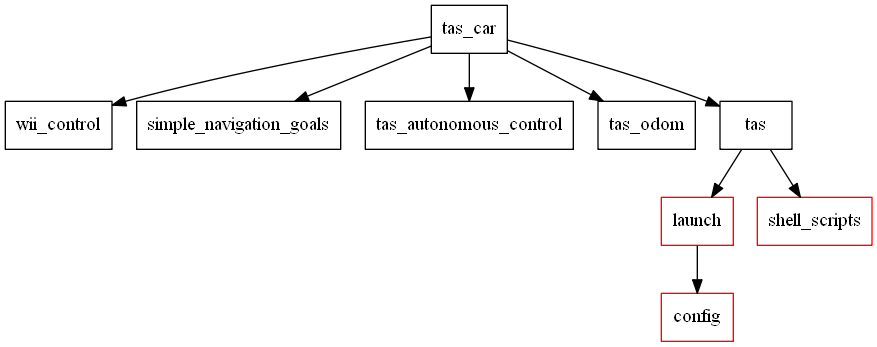
\includegraphics[width=\textwidth]{diagrams/tas_folder_struct}
	\caption{Folder structure of the TAS-package}
	\label{fig:tas_folder_struct}
\end{figure}

\newpage
\section{Installing the TAS-package}
\label{sec:tas_package_install 

As it was mentioned in the previous chapter the TAS-package can be found on GitHub. To install it open a terminal and switch to your catkin workspace directory. In this example we assume your working directory in \texttt{\textasciitilde/catkin\_ws}. To get and build the package on your car type in:

\shellcmd{cd \textasciitilde/catkin\_ws/src}\\
\shellcmd{git clone https://github.com/LSR-TAS/tas\_car}\\
\shellcmd{cd ..}\\
\shellcmd{catkin\_make}\\

If there occured no errors, the package has been built and the car is now ready to run. Before running anything you should also do the following preparations to make your work in the terminal a little more comfortable: 
\\
Open a terminal and type in:

\shellcmd{sudo gedit \textasciitilde/.bashrc}}

The \texttt{.bashrc} file is called automatically everytime you open a terminal in Ubuntu.
Add the following lines to the end of the textfile\footnote{Eventually you have to change the path of your catkin workspace directory}: 

\texttt{PATH=\textasciitilde/catkin\_ws/src/tas\_car/tas/shell\_scripts:"\$PATH"}\\
\texttt{source ros\_setup}\\

\todo{Add ros/opt..../setup.bash to ros\_setup file, and change file extension}

The first command will make it possible to run scripts from the specified folder without giving the full path. The second command sources the \texttt{ros\_setup} file from the \texttt{shell\_scripts} directory (see picture \reffig{tas_folder_struct} for the folder structure). This script mainly sets the correct access rights to read and write from the USB ports (see \ref{} for more detailed information).

\newpage
\section{Hardware drivers}
\label{sec:tas_package_drivers}

\begin{figure}[h]
	\centering
		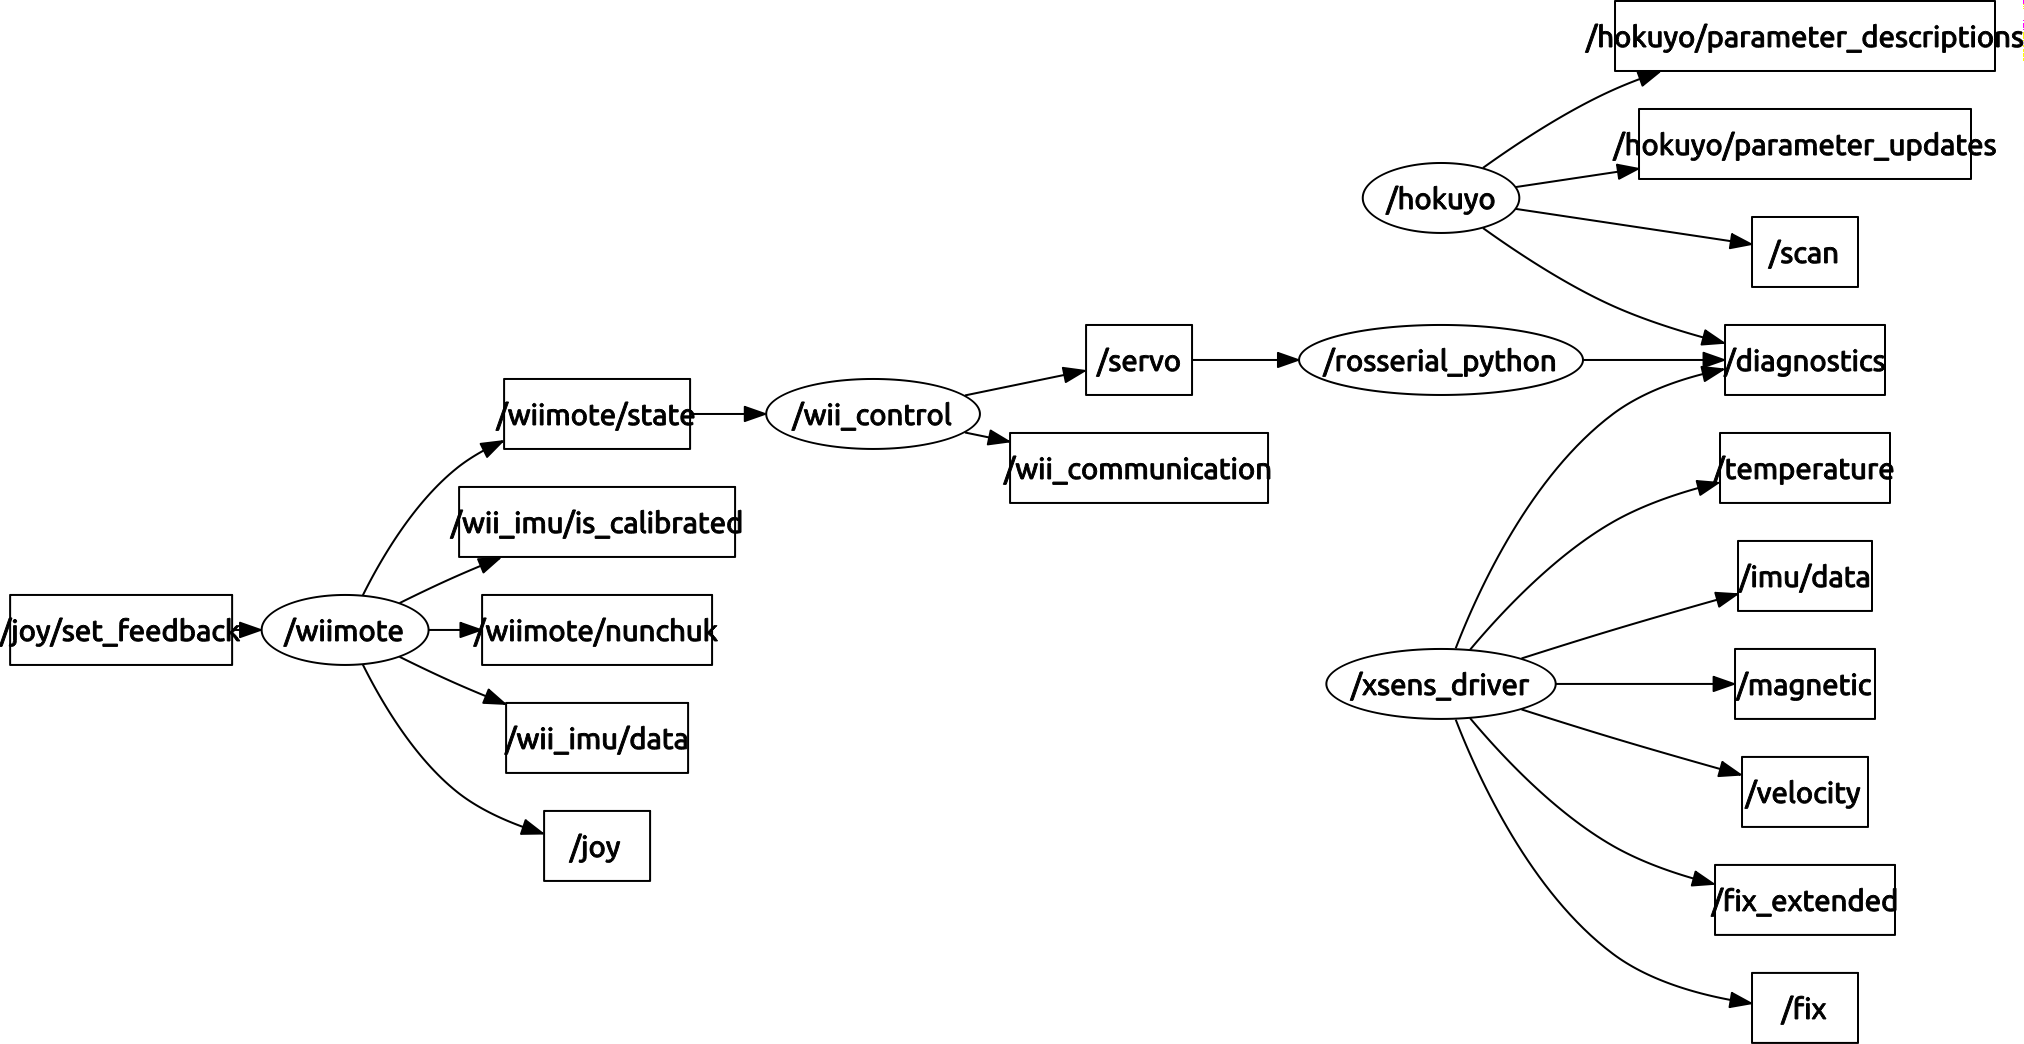
\includegraphics[width=0.9\textwidth]{diagrams/rqt_hardware}
	\caption{Overview of the hardware drivers}
	\label{fig:rqt_hardware}
\end{figure}

\begin{wrapfigure}{r}{0.13\textwidth}
  \begin{center}
    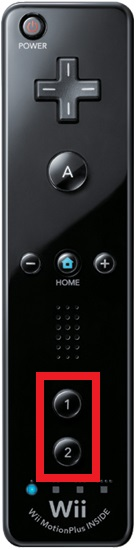
\includegraphics[width=0.13\textwidth]{wii}
		\label{fig:wii_controller}
  \end{center}	
\end{wrapfigure}

To run the hardware drivers open a terminal and type in:

\shellcmd{roscd tas/launch}\\
\shellcmd{roslaunch hardware.launch}

This will run several nodes to communicate with the hardware which will be explained in detail in the following sections. To establish the connection to the wii-controller press the the two two buttons at the bottom of the controller (see picture \reffig{wii_controller}) for about 5 seconds until you see a notification in the terminal window. The car now can be driven around manually.

In picture \reffig{rqt_hardware} you can see a graphical overview of the running nodes and topics. If you open a terminal and type in:

\shellcmd{rosrun rqt\_graph rqt\_graph}

you should get the same picture.


\subsection{wiimote}
\label{sec:tas_package_drivers_wiimote}
The \texttt{wiimote} node reads various data from the wii-controller via bluetooth and publishes it to the appropriate topic. We use these as control inputs for the car.

\hyperref[http://wiki.ros.org/wiimote?distro=indigo]{http://wiki.ros.org/wiimote?distro=indigo}

\subsection{wii\_control}
\label{sec:tas_package_drivers_wii_control}
The \texttt{wii\_control} node takes the inputs from the controller which are published by the \texttt{wiimote} node. From these inputs it calculates the PWM values for the motor controllers and publishes them to the \texttt{/servo} topic.


\subsection{rosserial\_python}
\label{sec:tas_package_drivers_rosserial}
The \texttt{rosserial\_python} node takes the PWM values from the \texttt{/servo} topic and sends them to the arduino. It mainly implements the communication channel between nodes and topics over a (virtual) serial port. For correct communication there has to be installed the so called \texttt{rosserial\_client} on the arduino. For more information refer to:

\hyperref[http://wiki.ros.org/rosserial]{http://wiki.ros.org/rosserial}

\subsection{hokuyo\_node}
\label{sec:tas_package_drivers_hokuyo}
The \texttt{hokuyo\_node} is the driver for the laserscanner. It reads the meausured data from the scanner via USB and publishes the to the \texttt{/scan} topic.

\hyperref[http://wiki.ros.org/hokuyo_node]{http://wiki.ros.org/hokuyo\_node}

\subsection{xsens\_driver}
\label{sec:tas_package_drivers_xsens}

The package provides a driver for several different IMUs from the XSens company. It reads data from the sensor via USB and publishes it to the \texttt{/imu/data} topic just like the \texttt{hokuyo\_node} does with the laser data.

\hyperref[http://wiki.ros.org/xsens_driver]{http://wiki.ros.org/xsens\_driver}

\newpage
\section{TAS-Odometry}
\label{sec:tas_package_odom}

\begin{figure}[h]
	\centering
		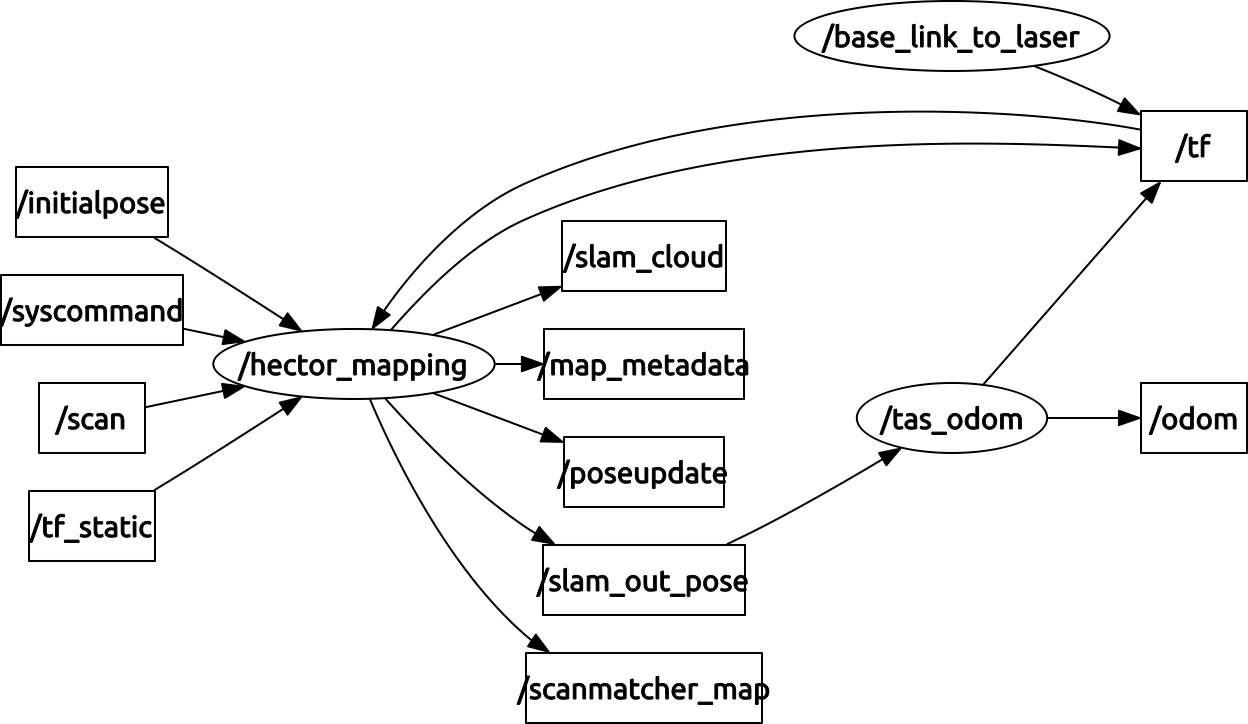
\includegraphics[width=0.9\textwidth]{diagrams/rqt_odom}
	\caption{Overview of the TAS-Odometry}
	\label{fig:rqt_odom}
\end{figure}

Currently there is no real odometry on the car available. For the navigation packages though odometry data is required (see picture \reffig{move_base_overview}). This was solved by implementation of a "fake-odometry". It uses position and orientation estimated from the laserscanner data, calculates the velocities and provides it as odometry data.

To launch the fake odometry open a terminal and run the odom.launch file:

\shellcmd{roscd tas/launch} \\
\shellcmd{roslaunch odom.launch}

Picture \reffig{rqt_odom} shows the running nodes and topics for the fake odometry.

\subsection{hector\_mapping}
\label{sec:tas_package_odom_hector}
The hector\_mapping node implements a SLAM-algorithm \footnote{Simultaneous Localization and Mapping} to build a map and localize the car in it simultaneously at runtime. Unlike other solutions for localization (see the \texttt{amcl package}  in section \refsec{tas_package_amcl}) it only needs data from the laserscanner and does not require any odometry inputs. 

The estimated position and orientation is published to the \texttt{/poseupdate} and the \texttt{/slam\_out\_pose} topics. The messages on the first topic additionally contain the covariances.
 
For correct calculation the node needs information about the relation between coordinate frame of the laserscanner and the coordinate frame of the car (refer to \refsec{tas_package_transformation} for an introduction to transformations and frames). 

For more details about the parameters and settings of the package see:

\hyperref[http://wiki.ros.org/hector_mapping]{http://wiki.ros.org/hector\_mapping}

\subsection{tas\_odom}
\label{sec:tas_package_odom_node}
The tas\_odom node subscribes to the \texttt{/slam\_out\_pose} topic (see previous chapter \refsec{tas_package_odom_hector}) and calculates the velocity from the estimated position by determining the difference quotient. Position, orientation and velocity is then published to the \texttt{/odom} topic. See the following page for information about the content of odometry messages:

\hyperref[http://docs.ros.org/indigo/api/nav_msgs/html/msg/Odometry.html]{http://docs.ros.org/indigo/api/nav\_msgs/html/msg/Odometry.html}

Additionally it publishes the transformation from the odometry coordinate frame to the frame of the car. See the next section for more details about transformations.

\todo{Velocity has to be in base\_link frame/tas\_odom publishes twist with velocity in odom frame}

\section{Transformations}
\label{sec:tas_package_transformations}

\newpage
\section{Navigation}
\label{sec:tas_package_navigation}

\begin{figure}[h]
	\centering
		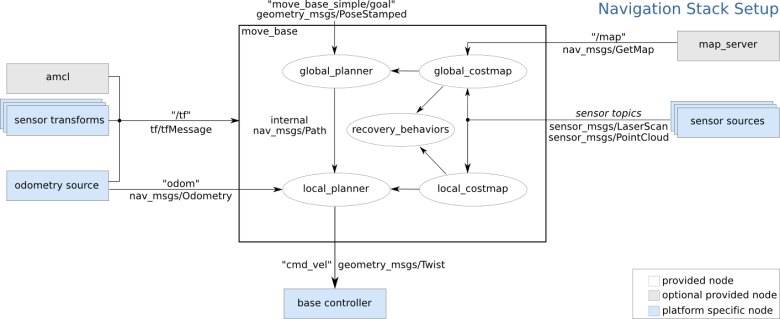
\includegraphics[width=\textwidth]{move_base_overview}
	\caption{Basic Navigation Stack}
	\label{fig:move_base_overview}
\end{figure}

In ROS in general the Navigation Stack takes sensor inputs from odometry, laser and other sources and outputs velocity commands to reach a given goal. Picture \reffig{move_base_overview} shows the parts of the basic Navigation Stack which is installed on the car.

To run the Navigation Stack open a terminal and type in:

\shellcmd{roscd tas/launch}\\
\shellcmd{roslaunch move\_base.launch}

The launch file will run all necessary parts of the Stack. Keep in mind that the hardware drivers and the TAS-Odometry package have to be launched before (see \ref{tas_package_drivers} for hardware drivers and \ref{tas_package_odom} for odometry).

To specify a goal for the car you can use the visualization tool RVIZ. Open a terminal and type in:

\shellcmd{roscd tas/launch} \\
\shellcmd{rosrun rviz rviz -d config/rviz/tas\_rviz.rviz}

This will run rviz with the configuration file in the \texttt{config} directory. At the beginning you have to give an initial estimation of the position to the \texttt{amcl node}. After that you can give goals to the \texttt{move\_base node} which the car will try to reach (see the marked buttons in picture \reffig{rviz_estimation}). To actually drive the car you have to push the \texttt{C-button} on the wii-nunchuk. 

\begin{figure}[h]
	\centering
		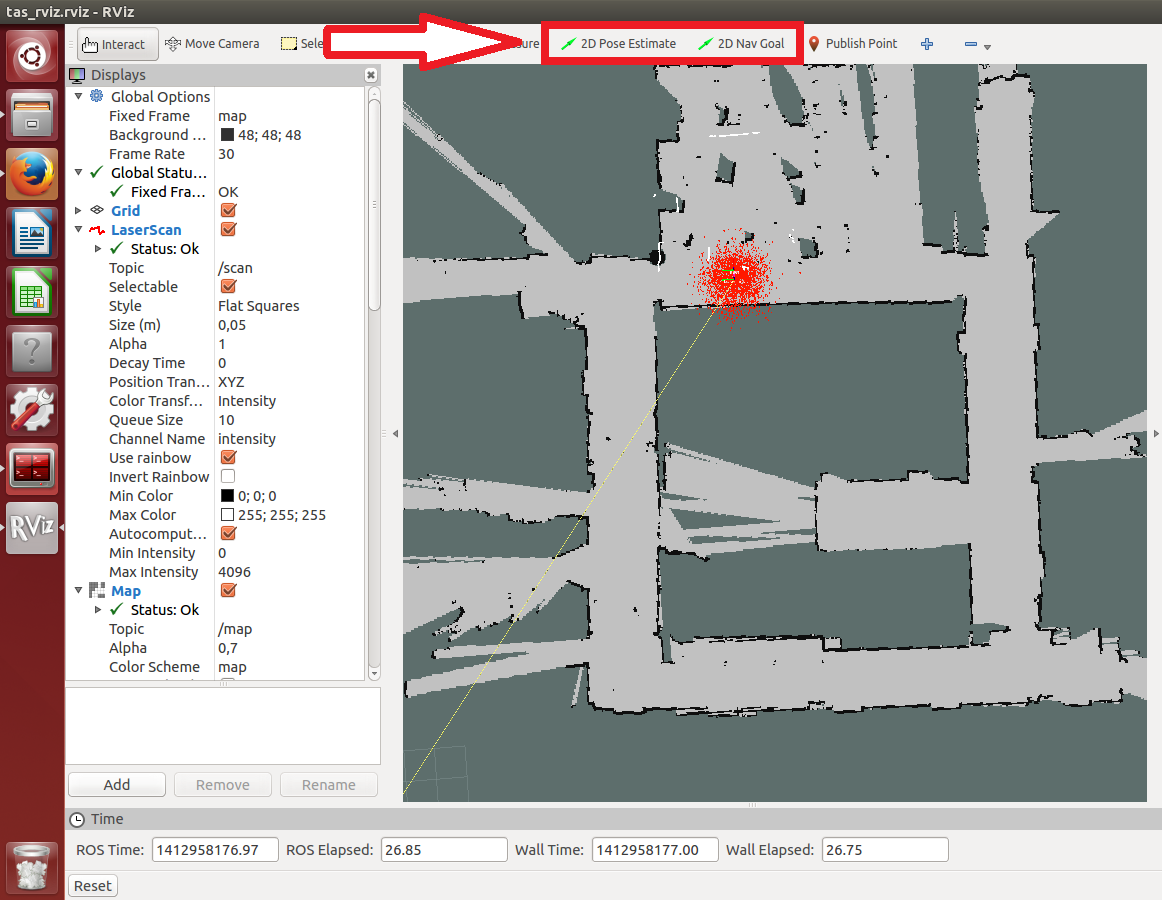
\includegraphics[width=\textwidth]{rviz_estimation}
	\caption{RVIZ visualization tool}
	\label{fig:rviz_estimation}
\end{figure}


Alternately you can launch hardware drivers, TAS-Odometry, the Navigation Stack and the RVIZ tool at once by launching the \texttt{run\_rviz.launch} file.

\subsection{map\_server}
\label{sec:tas_package_map_server}
The \texttt{map\_server} node takes a 2-D map of the environment and provides it as a ROS-service to other nodes. For every map there has to be a configuration file. The map file and the configuration file are located in the \texttt{config} directory of the TAS-package (see picture \reffig{} for the folder structure). The path of these files can be changed in the launchfile. For more information about the parameters of the \texttt{map\_server} package refer to:

\hyperref[http://wiki.ros.org/map_server]{http://wiki.ros.org/map_server}


\subsection{amcl}
\label{sec:tas_package_amcl}
The \texttt{amcl} node implements different Monte Carlo localization algorithms to estimate the position of the robot. It requires a laserscanner, odometry and a map of the environment. The position and orientation with it's covariances is published to the \texttt{/amcl\_pose} topic.

The node takes odometry data in form of the transformation between the odometry frame and the coordinate frame of the car. See section \refsec{} for information about the \texttt{tf package}. Refer also to the package documentation on:

\hyperref[http://wiki.ros.org/amcl]{http://wiki.ros.org/amcl}



\subsection{move\_base}
\label{sec:tas_package_move_base}

\subsection{tas\_autonomous\_control}
\label{sec:tas_package_autonomous_control}











